\documentclass[12pt,]{article}
\usepackage{lmodern}
\usepackage{amssymb,amsmath}
\usepackage{ifxetex,ifluatex}
\usepackage{fixltx2e} % provides \textsubscript
\ifnum 0\ifxetex 1\fi\ifluatex 1\fi=0 % if pdftex
  \usepackage[T1]{fontenc}
  \usepackage[utf8]{inputenc}
\else % if luatex or xelatex
  \ifxetex
    \usepackage{mathspec}
  \else
    \usepackage{fontspec}
  \fi
  \defaultfontfeatures{Ligatures=TeX,Scale=MatchLowercase}
    \setmainfont[]{Times New Roman}
\fi
% use upquote if available, for straight quotes in verbatim environments
\IfFileExists{upquote.sty}{\usepackage{upquote}}{}
% use microtype if available
\IfFileExists{microtype.sty}{%
\usepackage[]{microtype}
\UseMicrotypeSet[protrusion]{basicmath} % disable protrusion for tt fonts
}{}
\PassOptionsToPackage{hyphens}{url} % url is loaded by hyperref
\usepackage[unicode=true]{hyperref}
\hypersetup{
            pdftitle={Hydrological Characteristics of a Flood Event on the Lower Roanoke River},
            pdfauthor={Yingfan Zeng},
            pdfborder={0 0 0},
            breaklinks=true}
\urlstyle{same}  % don't use monospace font for urls
\usepackage[margin=2.54cm]{geometry}
\usepackage{longtable,booktabs}
% Fix footnotes in tables (requires footnote package)
\IfFileExists{footnote.sty}{\usepackage{footnote}\makesavenoteenv{long table}}{}
\usepackage{graphicx,grffile}
\makeatletter
\def\maxwidth{\ifdim\Gin@nat@width>\linewidth\linewidth\else\Gin@nat@width\fi}
\def\maxheight{\ifdim\Gin@nat@height>\textheight\textheight\else\Gin@nat@height\fi}
\makeatother
% Scale images if necessary, so that they will not overflow the page
% margins by default, and it is still possible to overwrite the defaults
% using explicit options in \includegraphics[width, height, ...]{}
\setkeys{Gin}{width=\maxwidth,height=\maxheight,keepaspectratio}
\IfFileExists{parskip.sty}{%
\usepackage{parskip}
}{% else
\setlength{\parindent}{0pt}
\setlength{\parskip}{6pt plus 2pt minus 1pt}
}
\setlength{\emergencystretch}{3em}  % prevent overfull lines
\providecommand{\tightlist}{%
  \setlength{\itemsep}{0pt}\setlength{\parskip}{0pt}}
\setcounter{secnumdepth}{5}
% Redefines (sub)paragraphs to behave more like sections
\ifx\paragraph\undefined\else
\let\oldparagraph\paragraph
\renewcommand{\paragraph}[1]{\oldparagraph{#1}\mbox{}}
\fi
\ifx\subparagraph\undefined\else
\let\oldsubparagraph\subparagraph
\renewcommand{\subparagraph}[1]{\oldsubparagraph{#1}\mbox{}}
\fi

% set default figure placement to htbp
\makeatletter
\def\fps@figure{htbp}
\makeatother

\usepackage{etoolbox}
\makeatletter
\providecommand{\subtitle}[1]{% add subtitle to \maketitle
  \apptocmd{\@title}{\par {\large #1 \par}}{}{}
}
\makeatother

\title{Hydrological Characteristics of a Flood Event on the Lower Roanoke River}
\providecommand{\subtitle}[1]{}
\subtitle{\url{https://github.com/YFZeng07/ENV790_WDA_FinalProject.git}}
\author{Yingfan Zeng}
\date{}

\begin{document}
\maketitle

\newpage

\section{Rationale and Research
Questions}\label{rationale-and-research-questions}

Flooding is one of the most dangerous natural disasters in the world,
affecting societies, economies, and ecosystems. With climate change,
floods are increasing in intensity and frequency (Bates, Kundzewicz, Wu,
\& Palutikof, 2008). Flooding is the main stressor for many ecosystems
like forests. Globally speaking, there is a strong link between
increased flood frequency and forest loss, as well as the intensity and
duration of floods (Bradshaw, Sodhi, PEH, \& Brook, 2007). Lower Roanoke
River Basin has one of the most biodiverse ecosystems in the Southeast
United States. It is a typical southeastern alluvial system, contains
the largest natural bottomland hardwood forests in the mid-Atlantic
region, and is home to a massive number of fish and wildlife species
(U.S. Fish \& Wildlife Service, 2014). However, forests on Roanoke
floodplains have been threatened by flooding there is a strong negative
correlation between the vegetation species composition and tree growth
rate (Townsend, 2001). Given the lack of study on hydrology
characteristics of the Roanoke River flooding, this project selected a
specific flood event to investigate the following questions:

\begin{enumerate}
\def\labelenumi{\arabic{enumi}.}
\tightlist
\item
  How long was the flood duration along the river?
\item
  How was the water height change during a flood event?
\item
  How did the flood peak move along the river?
\end{enumerate}

\newpage

\section{Dataset Information}\label{dataset-information}

\subsection{Study Area}\label{study-area}

The Lower Roanoke River Basin is in southern Virginia and northeastern
North Carolina in the United States. Located between the John H. Kerr
Dam and the Albemarle Sound, this 600000-ha basin contains over 200 km
of the Roanoke River, with floodplains of about 5-10 km in width. There
is more than 25000 ha of floodplain forests in the basin (Townsend,
2001), which are deeply affected by the floods of the Roanoke River.

\subsection{Study Period}\label{study-period}

The discharge of upstream dams is closely related to downstream flooding
in the Lower Roanoke Watershed. There are 3 dams upstream from the study
area and they have a great impact on the basin: the John H. Kerr Dam,
the Gaston Dam, and the Roanoke Rapids Dam. There is no major dam below
the Roanoke Rapids Dam and its maximum discharge capacity is 20,000
cubic feet per second (cfs). Therefore, in this study, a flood event was
defined as a continuous period of the discharge of the Roanoke Rapids
Dam above 20,000 cfs. Because it had the largest dam discharge of 35000
cfs, I chose the flooding event between February 27 and March 11, 2019
to examine its hydrological characteristics.

\subsection{Water Height Data}\label{water-height-data}

Water height data from USGS gages along the Lower Roanoke River were
obtained to characterize the flooding hydrology for this flood event.
There are 8 USGS gages on Roanoke River from Roanoke Rapids to the
Albemarle Sound (Table 1, Figure 1). Their daily water height between
2/1/2019 and 4/5/2019 was retrieved to cover the flooding period.

\begin{longtable}[]{@{}lllrr@{}}
\caption{Table 1. The 8 USGS gages on the Lower Roanoke
River}\tabularnewline
\toprule
Agency & Gage ID & Gage Name & Latitude & Longitude\tabularnewline
\midrule
\endfirsthead
\toprule
Agency & Gage ID & Gage Name & Latitude & Longitude\tabularnewline
\midrule
\endhead
USGS & 02080500 & ROANOKE RIVER AT ROANOKE RAPIDS, NC & 36.46000 &
-77.63361\tabularnewline
USGS & 0208062765 & ROANOKE RIVER AT HALIFAX, NC & 36.33111 &
-77.58028\tabularnewline
USGS & 02081000 & ROANOKE RIVER NEAR SCOTLAND NECK, NC & 36.20917 &
-77.38389\tabularnewline
USGS & 02081022 & ROANOKE RIVER NEAR OAK CITY, NC & 36.01361 &
-77.21528\tabularnewline
USGS & 02081028 & ROANOKE RIVER AT HAMILTON, NC & 35.94750 &
-77.20250\tabularnewline
USGS & 02081054 & ROANOKE RIVER AT WILLIAMSTON, NC & 35.85972 &
-77.04028\tabularnewline
USGS & 02081094 & ROANOKE RIVER AT JAMESVILLE, NC & 35.81306 &
-76.89278\tabularnewline
USGS & 0208114150 & ROANOKE RIVER AT NC 45 NR WESTOVER, NC & 35.91500 &
-76.72278\tabularnewline
\bottomrule
\end{longtable}

\begin{figure}
\centering
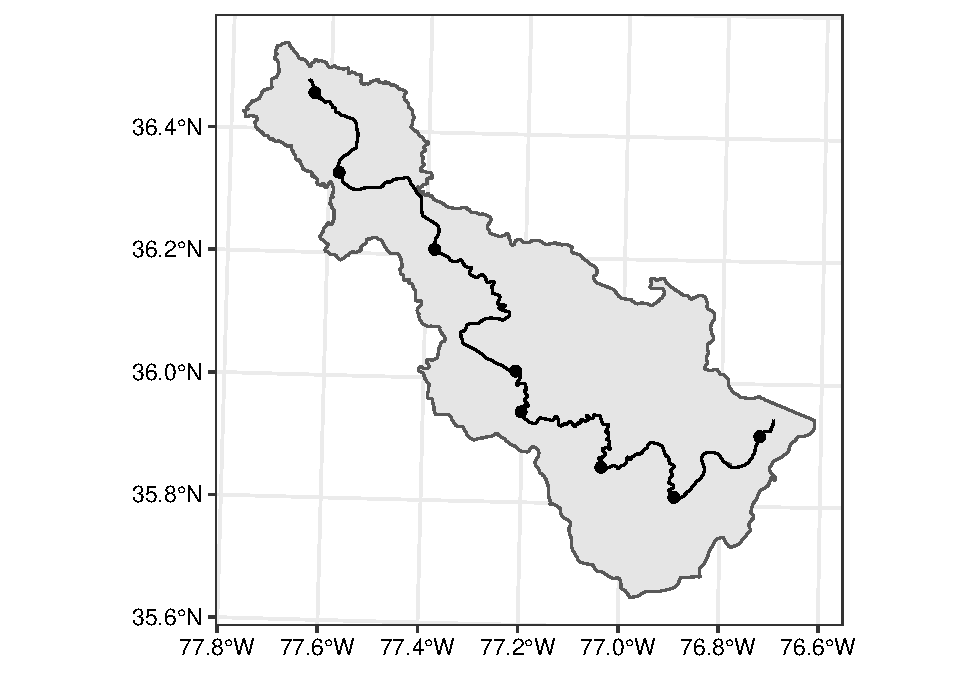
\includegraphics{Zeng_WDA_Project_files/figure-latex/Figure 1-1.pdf}
\caption{The Lower Roanoke River, its basin and the 8 USGS gages on it.}
\end{figure}

\newpage

\section{Exploratory Analysis}\label{exploratory-analysis}

To gain a general understanding of how water height changed during and
after the flood event, I plotted the water height for each gage from
upstream to downstream. For most of the gages, the data were too
volatile for subsequent analysis. Thus, I calculated the 5-day moving
average water height to smooth the trend. The comparison between the
original data and the 5-day average as well as the basic changes in
water level at each gage is shown in Figure 2.

\begin{figure}
\centering
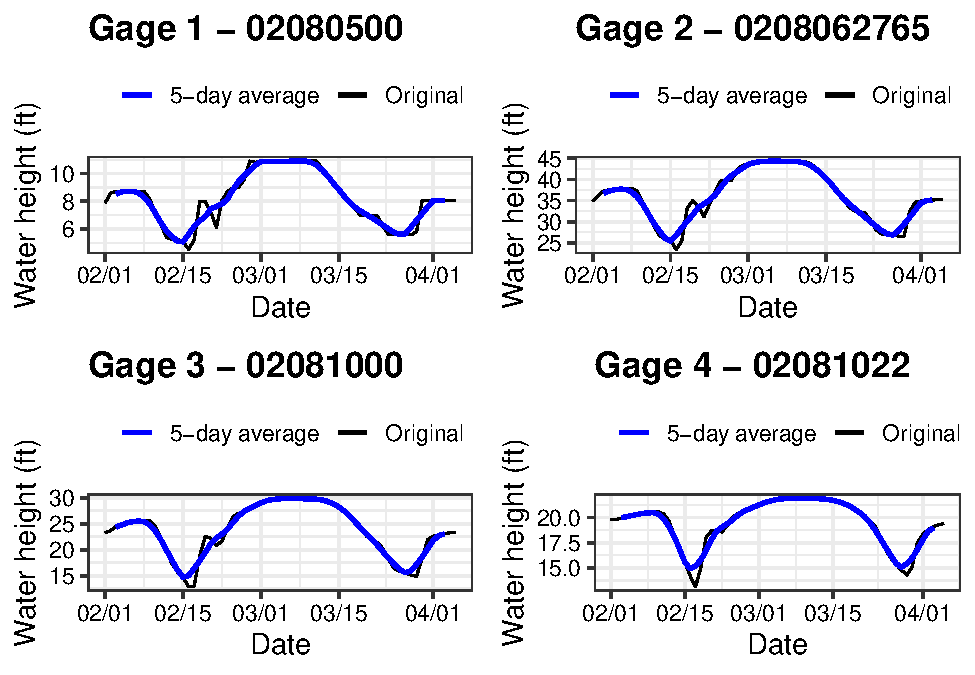
\includegraphics{Zeng_WDA_Project_files/figure-latex/Figure 2.1-1.pdf}
\caption{The water height changes during the flood event at Gage 1-4}
\end{figure}

\begin{figure}
\centering
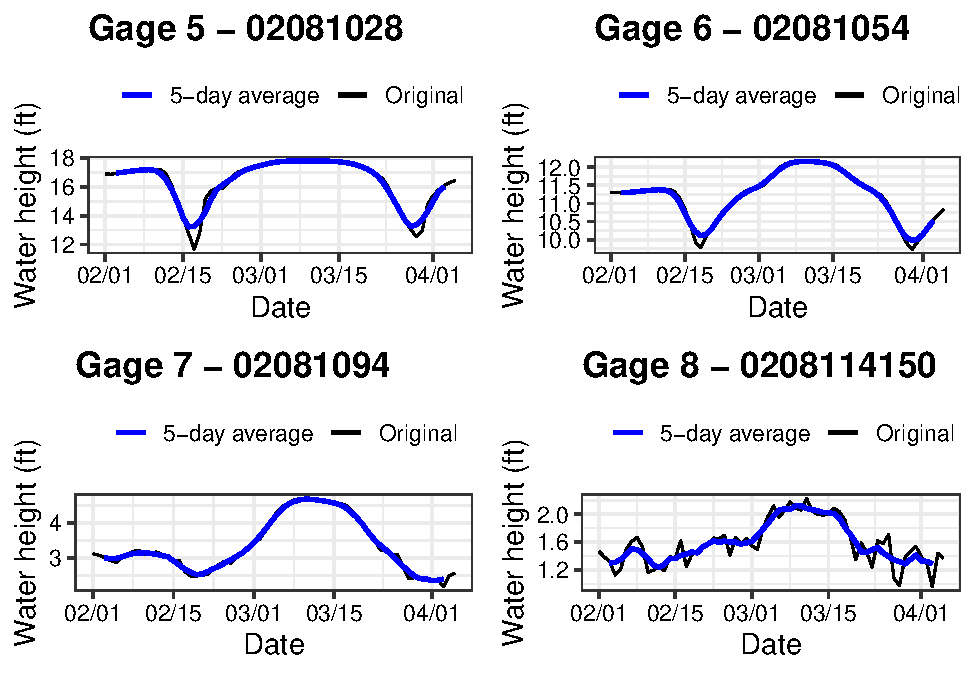
\includegraphics{Zeng_WDA_Project_files/figure-latex/Figure 2.2-1.pdf}
\caption{The water height changes during the flood event at Gage 5-8}
\end{figure}

\newpage

\section{Analysis}\label{analysis}

The flooding hydrology of this flood event on the Lower Roanoke River
was characterized by 3 values: flood duration, water height change rate,
and flood peak moving speed. I defined the start date as the first day
the water height started to increase, and the end date as the last day
the water height decreased after the pulse. The flood duration was
determined by the day difference between the start date and the end
date. Then, I selected the maximum water level and the lowest water
level (normally the first day) during the flooding period and calculated
the water height change rate as (maximum level -- minimum level)/minimum
level. The day with the maximum water height was considered as the flood
peak date, and the flood peak day difference at each gage along the
river was analyzed. The results were visualized on maps by color
gradients.

\begin{longtable}[]{@{}ccccc@{}}
\caption{Table 2. The hydrological characteristics at the 8 USGS gages
on the Lower Roanoke River (continued below)}\tabularnewline
\toprule
\begin{minipage}[b]{0.10\columnwidth}\centering\strut
Agency\strut
\end{minipage} & \begin{minipage}[b]{0.15\columnwidth}\centering\strut
Gage ID\strut
\end{minipage} & \begin{minipage}[b]{0.36\columnwidth}\centering\strut
Gage Name\strut
\end{minipage} & \begin{minipage}[b]{0.12\columnwidth}\centering\strut
Latitude\strut
\end{minipage} & \begin{minipage}[b]{0.12\columnwidth}\centering\strut
Longitude\strut
\end{minipage}\tabularnewline
\midrule
\endfirsthead
\toprule
\begin{minipage}[b]{0.10\columnwidth}\centering\strut
Agency\strut
\end{minipage} & \begin{minipage}[b]{0.15\columnwidth}\centering\strut
Gage ID\strut
\end{minipage} & \begin{minipage}[b]{0.36\columnwidth}\centering\strut
Gage Name\strut
\end{minipage} & \begin{minipage}[b]{0.12\columnwidth}\centering\strut
Latitude\strut
\end{minipage} & \begin{minipage}[b]{0.12\columnwidth}\centering\strut
Longitude\strut
\end{minipage}\tabularnewline
\midrule
\endhead
\begin{minipage}[t]{0.10\columnwidth}\centering\strut
USGS\strut
\end{minipage} & \begin{minipage}[t]{0.15\columnwidth}\centering\strut
02080500\strut
\end{minipage} & \begin{minipage}[t]{0.36\columnwidth}\centering\strut
ROANOKE RIVER AT ROANOKE RAPIDS, NC\strut
\end{minipage} & \begin{minipage}[t]{0.12\columnwidth}\centering\strut
36.46\strut
\end{minipage} & \begin{minipage}[t]{0.12\columnwidth}\centering\strut
-77.63\strut
\end{minipage}\tabularnewline
\begin{minipage}[t]{0.10\columnwidth}\centering\strut
USGS\strut
\end{minipage} & \begin{minipage}[t]{0.15\columnwidth}\centering\strut
0208062765\strut
\end{minipage} & \begin{minipage}[t]{0.36\columnwidth}\centering\strut
ROANOKE RIVER AT HALIFAX, NC\strut
\end{minipage} & \begin{minipage}[t]{0.12\columnwidth}\centering\strut
36.33\strut
\end{minipage} & \begin{minipage}[t]{0.12\columnwidth}\centering\strut
-77.58\strut
\end{minipage}\tabularnewline
\begin{minipage}[t]{0.10\columnwidth}\centering\strut
USGS\strut
\end{minipage} & \begin{minipage}[t]{0.15\columnwidth}\centering\strut
02081000\strut
\end{minipage} & \begin{minipage}[t]{0.36\columnwidth}\centering\strut
ROANOKE RIVER NEAR SCOTLAND NECK, NC\strut
\end{minipage} & \begin{minipage}[t]{0.12\columnwidth}\centering\strut
36.21\strut
\end{minipage} & \begin{minipage}[t]{0.12\columnwidth}\centering\strut
-77.38\strut
\end{minipage}\tabularnewline
\begin{minipage}[t]{0.10\columnwidth}\centering\strut
USGS\strut
\end{minipage} & \begin{minipage}[t]{0.15\columnwidth}\centering\strut
02081022\strut
\end{minipage} & \begin{minipage}[t]{0.36\columnwidth}\centering\strut
ROANOKE RIVER NEAR OAK CITY, NC\strut
\end{minipage} & \begin{minipage}[t]{0.12\columnwidth}\centering\strut
36.01\strut
\end{minipage} & \begin{minipage}[t]{0.12\columnwidth}\centering\strut
-77.22\strut
\end{minipage}\tabularnewline
\begin{minipage}[t]{0.10\columnwidth}\centering\strut
USGS\strut
\end{minipage} & \begin{minipage}[t]{0.15\columnwidth}\centering\strut
02081028\strut
\end{minipage} & \begin{minipage}[t]{0.36\columnwidth}\centering\strut
ROANOKE RIVER AT HAMILTON, NC\strut
\end{minipage} & \begin{minipage}[t]{0.12\columnwidth}\centering\strut
35.95\strut
\end{minipage} & \begin{minipage}[t]{0.12\columnwidth}\centering\strut
-77.2\strut
\end{minipage}\tabularnewline
\begin{minipage}[t]{0.10\columnwidth}\centering\strut
USGS\strut
\end{minipage} & \begin{minipage}[t]{0.15\columnwidth}\centering\strut
02081054\strut
\end{minipage} & \begin{minipage}[t]{0.36\columnwidth}\centering\strut
ROANOKE RIVER AT WILLIAMSTON, NC\strut
\end{minipage} & \begin{minipage}[t]{0.12\columnwidth}\centering\strut
35.86\strut
\end{minipage} & \begin{minipage}[t]{0.12\columnwidth}\centering\strut
-77.04\strut
\end{minipage}\tabularnewline
\begin{minipage}[t]{0.10\columnwidth}\centering\strut
USGS\strut
\end{minipage} & \begin{minipage}[t]{0.15\columnwidth}\centering\strut
02081094\strut
\end{minipage} & \begin{minipage}[t]{0.36\columnwidth}\centering\strut
ROANOKE RIVER AT JAMESVILLE, NC\strut
\end{minipage} & \begin{minipage}[t]{0.12\columnwidth}\centering\strut
35.81\strut
\end{minipage} & \begin{minipage}[t]{0.12\columnwidth}\centering\strut
-76.89\strut
\end{minipage}\tabularnewline
\begin{minipage}[t]{0.10\columnwidth}\centering\strut
USGS\strut
\end{minipage} & \begin{minipage}[t]{0.15\columnwidth}\centering\strut
0208114150\strut
\end{minipage} & \begin{minipage}[t]{0.36\columnwidth}\centering\strut
ROANOKE RIVER AT NC 45 NR WESTOVER, NC\strut
\end{minipage} & \begin{minipage}[t]{0.12\columnwidth}\centering\strut
35.91\strut
\end{minipage} & \begin{minipage}[t]{0.12\columnwidth}\centering\strut
-76.72\strut
\end{minipage}\tabularnewline
\bottomrule
\end{longtable}

\begin{longtable}[]{@{}ccccc@{}}
\toprule
\begin{minipage}[b]{0.14\columnwidth}\centering\strut
Start date\strut
\end{minipage} & \begin{minipage}[b]{0.14\columnwidth}\centering\strut
End date\strut
\end{minipage} & \begin{minipage}[b]{0.14\columnwidth}\centering\strut
Peak date\strut
\end{minipage} & \begin{minipage}[b]{0.12\columnwidth}\centering\strut
Duration\strut
\end{minipage} & \begin{minipage}[b]{0.30\columnwidth}\centering\strut
Water level increase rate\strut
\end{minipage}\tabularnewline
\midrule
\endhead
\begin{minipage}[t]{0.14\columnwidth}\centering\strut
2019-02-15\strut
\end{minipage} & \begin{minipage}[t]{0.14\columnwidth}\centering\strut
2019-03-26\strut
\end{minipage} & \begin{minipage}[t]{0.14\columnwidth}\centering\strut
2019-03-08\strut
\end{minipage} & \begin{minipage}[t]{0.12\columnwidth}\centering\strut
39\strut
\end{minipage} & \begin{minipage}[t]{0.30\columnwidth}\centering\strut
1.15\strut
\end{minipage}\tabularnewline
\begin{minipage}[t]{0.14\columnwidth}\centering\strut
2019-02-15\strut
\end{minipage} & \begin{minipage}[t]{0.14\columnwidth}\centering\strut
2019-03-27\strut
\end{minipage} & \begin{minipage}[t]{0.14\columnwidth}\centering\strut
2019-03-06\strut
\end{minipage} & \begin{minipage}[t]{0.12\columnwidth}\centering\strut
40\strut
\end{minipage} & \begin{minipage}[t]{0.30\columnwidth}\centering\strut
0.7478\strut
\end{minipage}\tabularnewline
\begin{minipage}[t]{0.14\columnwidth}\centering\strut
2019-02-16\strut
\end{minipage} & \begin{minipage}[t]{0.14\columnwidth}\centering\strut
2019-03-27\strut
\end{minipage} & \begin{minipage}[t]{0.14\columnwidth}\centering\strut
2019-03-06\strut
\end{minipage} & \begin{minipage}[t]{0.12\columnwidth}\centering\strut
39\strut
\end{minipage} & \begin{minipage}[t]{0.30\columnwidth}\centering\strut
0.9864\strut
\end{minipage}\tabularnewline
\begin{minipage}[t]{0.14\columnwidth}\centering\strut
2019-02-17\strut
\end{minipage} & \begin{minipage}[t]{0.14\columnwidth}\centering\strut
2019-03-28\strut
\end{minipage} & \begin{minipage}[t]{0.14\columnwidth}\centering\strut
2019-03-08\strut
\end{minipage} & \begin{minipage}[t]{0.12\columnwidth}\centering\strut
39\strut
\end{minipage} & \begin{minipage}[t]{0.30\columnwidth}\centering\strut
0.4512\strut
\end{minipage}\tabularnewline
\begin{minipage}[t]{0.14\columnwidth}\centering\strut
2019-02-17\strut
\end{minipage} & \begin{minipage}[t]{0.14\columnwidth}\centering\strut
2019-03-28\strut
\end{minipage} & \begin{minipage}[t]{0.14\columnwidth}\centering\strut
2019-03-08\strut
\end{minipage} & \begin{minipage}[t]{0.12\columnwidth}\centering\strut
39\strut
\end{minipage} & \begin{minipage}[t]{0.30\columnwidth}\centering\strut
0.3445\strut
\end{minipage}\tabularnewline
\begin{minipage}[t]{0.14\columnwidth}\centering\strut
2019-02-19\strut
\end{minipage} & \begin{minipage}[t]{0.14\columnwidth}\centering\strut
2019-03-30\strut
\end{minipage} & \begin{minipage}[t]{0.14\columnwidth}\centering\strut
2019-03-10\strut
\end{minipage} & \begin{minipage}[t]{0.12\columnwidth}\centering\strut
39\strut
\end{minipage} & \begin{minipage}[t]{0.30\columnwidth}\centering\strut
0.2191\strut
\end{minipage}\tabularnewline
\begin{minipage}[t]{0.14\columnwidth}\centering\strut
2019-02-20\strut
\end{minipage} & \begin{minipage}[t]{0.14\columnwidth}\centering\strut
2019-04-01\strut
\end{minipage} & \begin{minipage}[t]{0.14\columnwidth}\centering\strut
2019-03-10\strut
\end{minipage} & \begin{minipage}[t]{0.12\columnwidth}\centering\strut
40\strut
\end{minipage} & \begin{minipage}[t]{0.30\columnwidth}\centering\strut
0.9983\strut
\end{minipage}\tabularnewline
\begin{minipage}[t]{0.14\columnwidth}\centering\strut
2019-03-01\strut
\end{minipage} & \begin{minipage}[t]{0.14\columnwidth}\centering\strut
2019-04-05\strut
\end{minipage} & \begin{minipage}[t]{0.14\columnwidth}\centering\strut
2019-03-09\strut
\end{minipage} & \begin{minipage}[t]{0.12\columnwidth}\centering\strut
35\strut
\end{minipage} & \begin{minipage}[t]{0.30\columnwidth}\centering\strut
0.6698\strut
\end{minipage}\tabularnewline
\bottomrule
\end{longtable}

\begin{figure}
\centering
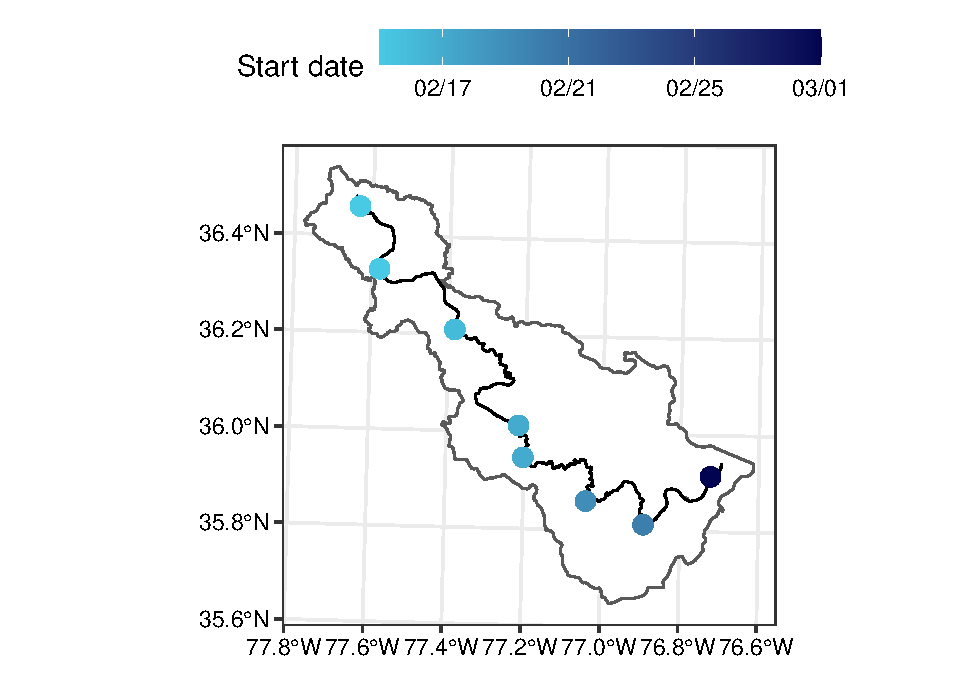
\includegraphics{Zeng_WDA_Project_files/figure-latex/Figure 3-1.pdf}
\caption{The start date of the flood event at each gages.}
\end{figure}

\begin{figure}
\centering
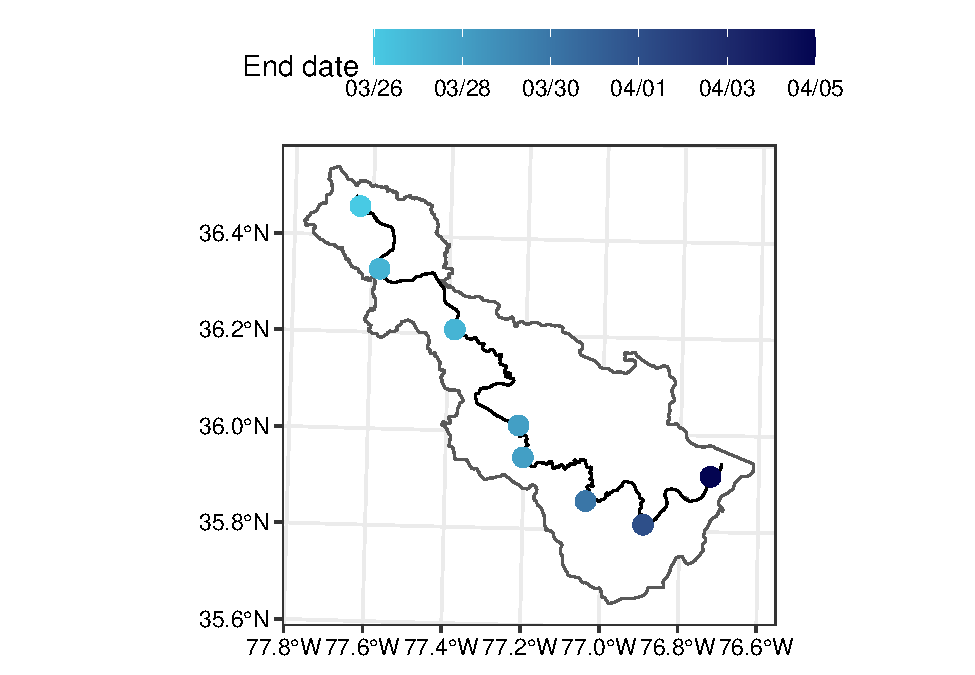
\includegraphics{Zeng_WDA_Project_files/figure-latex/Figure 4-1.pdf}
\caption{The end date of the flood event at each gages.}
\end{figure}

\begin{figure}
\centering
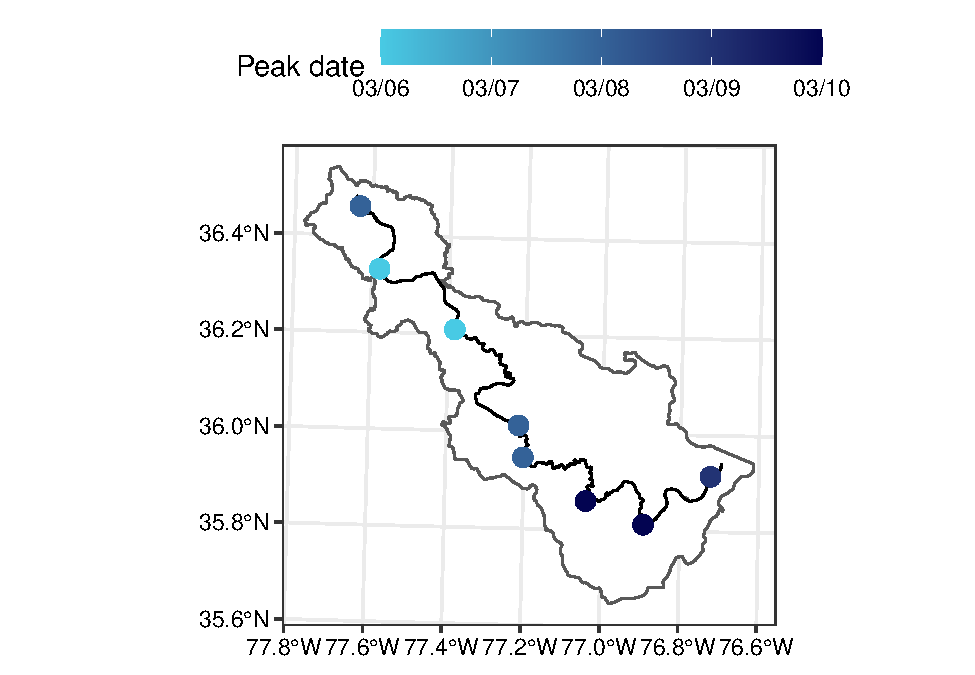
\includegraphics{Zeng_WDA_Project_files/figure-latex/Figure 5-1.pdf}
\caption{The peak date of the flood event at each gages.}
\end{figure}

\begin{figure}
\centering
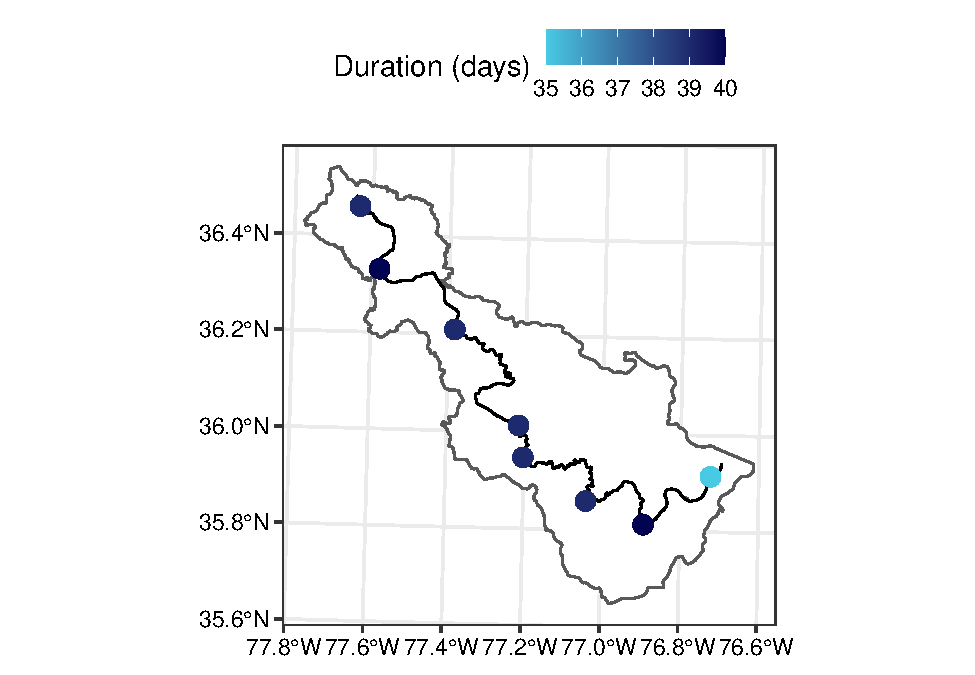
\includegraphics{Zeng_WDA_Project_files/figure-latex/Figure 6-1.pdf}
\caption{The duration of the flood event at each gages.}
\end{figure}

\begin{figure}
\centering
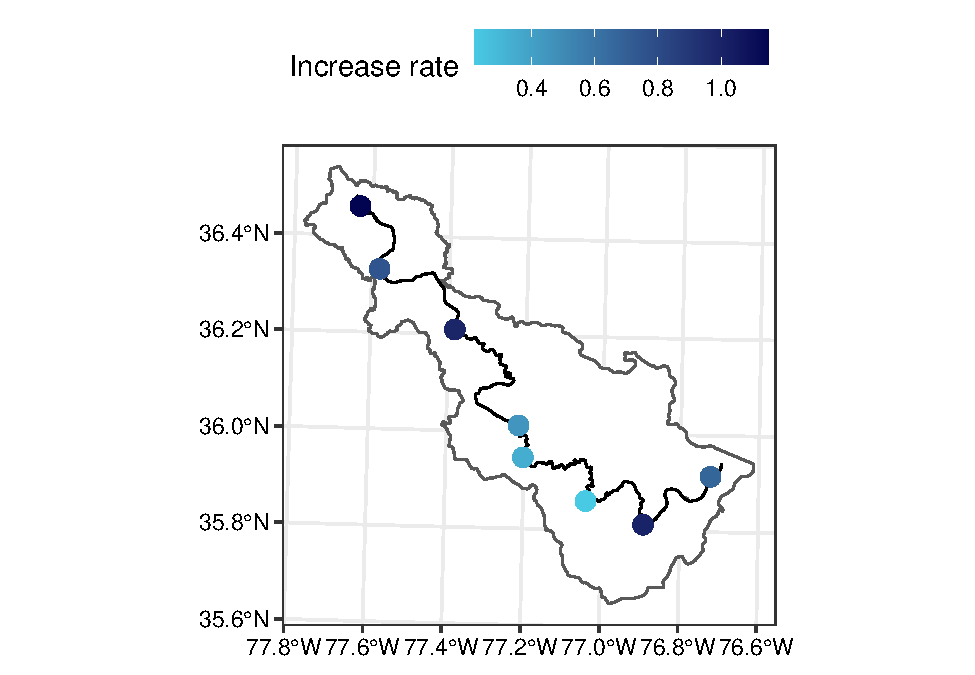
\includegraphics{Zeng_WDA_Project_files/figure-latex/Figure 7-1.pdf}
\caption{The water level increase rate of the flood event at each
gages.}
\end{figure}

\newpage

\section{Summary and Conclusions}\label{summary-and-conclusions}

The flood duration ranged between 35 and 40 days at the 8 gages along
the river. There was not much spatial trend on flood duration. Except
for the most downstream Gage 8, the flood duration of the other gages
was 39 or 40 days. This indicated that there was no discernible spatial
difference in duration along the river as the flood flowed downstream.
By the time it reached the most downstream, much of the water might have
been consumed, so the length of the flood at the most downstream gage
was significantly shorter.

Although the peak dates were close, the flood start and end dates varied
at each gage. The flooding period at the most downstream site (Gage 8)
was 15 days later than the most upstream gage at the dam (Gage 1), and
the second-to-last downstream point (Gage 7) also had a 5-day lag. It
took about 5 days for the water to flow from the upstream to the
downstream, meaning that the downstream should expect the flood to
arrive 5 days after the dam discharging started.

During a flood event, water level increase rates were high upstream and
downstream, but low in the middle of the basin. The most upstream gage
at the dam had the highest water level increase of 115\%, while the
lowest increase rate on the river was only 21\% at Gage 6. The water
level in the upper and lower reaches had increased by about 70\% or
more, while in the middle river there was only about 45\% or less. This
might be due to the narrow channels in the upper and lower reaches, with
wide channels and broad floodplains in the middle basin. In fact, a
lower water level increase rate might mean more overbank flow and more
severe flooding.

In conclusion, for the flood event in March 2019, the duration at
different locations along the river was similar, while there was about a
5-day lag of the flooding period from upstream to downstream. The water
level increased more in the most upstream and downstream areas, and less
in the middle basin. This study deepened the understanding of flooding
hydrology on the Lower Roanoke River and could serve as a reference for
future flood prevention and control.

\newpage

\section{References}\label{references}

Bates, B. C., Kundzewicz, Z. W., Wu, S., \& Palutikof, J. P. (2008).
Climate Change and Water. Technical Paper of the Intergovernmental Panel
on Climate Change, IPCC Secretariat: Geneva, Switzerland. The American
Midland Naturalist, 168(1).

Bradshaw, C. J., Sodhi, N. S., PEH, K. S. H., \& Brook, B. W. (2007).
Global evidence that deforestation amplifies flood risk and severity in
the developing world. Global Change Biology, 13(11), 2379-2395.

U.S. Fish \& Wildlife Service. (2014). National Wildlife Refuge: Roanoke
River.
\url{https://www.fws.gov/refuge/Roanoke_River/wildlife_and_habitat/index.html}

Townsend, P. A. (2001). Relationships between vegetation patterns and
hydroperiod on the Roanoke River floodplain, North Carolina. Plant
Ecology, 156(1), 43-58.

\end{document}
